\chapter{Υλικό \& λογισμικό}
\label{chapter:architecture}
% about this chapter ~2 paragraphs
Στο κεφάλαιο αυτό παρουσιάζονται τα βασικά εργαλεία που χρησιμοποιήθηκαν
τόσο για τις υλοποιήσεις όσο και για τα πειράματα. Η αναφορά αυτή γίνεται για τον ερευνητή ο οποίος θέλει να εξετάσει λεπτομέρειες της υλοποίησης. Όλα τα σχετικά αρχεία και ο κώδικας βρίσκεται στο \footnote{\url{https://github.com/supernlogn/SqueezeDetTL}}. Στην ενότητα \ref{section:hardware} παρουσιάζεται το υλικό πάνω στο οποίο βασίστηκε η εργασία, ενώ στην ενότητα \ref{section:software} παρουσιάζεται η δόμηση του λογισμικού και τα εργαλεία που χρησιμοποιήθηκαν.

\section{Περιγραφή του υλικού}
\label{section:hardware}
Η παρούσα διπλωματική έγινε στην υπολογιστική συστοιχία του εργαστηρίου Αρχιτεκτονικής Υπολογιστών και Συστημάτων. Τα κύρια μέρη της συστοιχίας που αφορούν είναι 1) η CPU 2) η GPU 3) RAM και ο σκληρός δίσκος. Για περισσότερες λεπτομέρειες, επειδή σε μελλοντικά πειράματα μπορεί να υπάρχουν επιπλέον παράμετροι υλικού, ολόκληρη η ανάλυση του υλικού της συστοιχίας παρατίθεται σε έναν υπερσύνδεσμο\footnote{\url{https://drive.google.com/file/d/1c7IuY3qEbz3VoLnWaWf4ZrtjjNa5O1Rf/view?usp=sharing}}.

\begin{enumerate}
    \item CPU: Intel(R) Core(TM) i7-7700K CPU @ 4.20GHz \footnote{\url{https://ark.intel.com/products/97129/Intel-Core-i7-7700K-Processor-8M-Cache-up-to-4_50-GHz}}
    \item GPU: NVIDIA GEFORCE GTX 1080 Ti \footnote{\url{https://www.nvidia.com/en-us/geforce/products/10series/geforce-gtx-1080-ti/}}
    \item RAM: $2 \times$ DIMM Synchronous 2400 MHz, 8GiB, 64 bits
    \item hard drive: ATA Disk HDD(για τα σύνολα δεδομένων και τα αποτελέσματα) $+$ ATA Disk SSD (για αποθήκευση του κώδικα) 
\end{enumerate}

\section{Βασικά στοιχεία δόμησης λογισμικού}
\label{section:software}
Σε αυτή την ενότητα παρουσιάζονται τα δύο βασικότερα κομμάτια της δόμησης του λογισμικού και τα πακέτα λογισμικού τρίτων.

\subsection{Περιγραφή της δόμησης}
Τα δομικά στοιχεία της συνολικής υλοποίησης είναι εμπνευσμένα από το σχήμα 24 στο βιβλίο νευρωνικών δικτύων του Haykin \cite{66}. Η εικόνα αυτή διαφοροποιημένη φαίνεται στο Σχήμα \ref{fig:haykin_figure}. Εκεί παρουσιάζεται οπτικά και ο τρόπος λειτουργίας της υλοποίησης. Σύμφωνα με αυτή ορίζονται τα δύο μπλοκ \textit{supervisor} και \textit{hypervisor} τα οποία υλοποιούνται στα ομώνυμα πακέτα. Τα δύο αυτά πακέτα αναλύονται παρακάτω.

\begin{figure}
    \centering
    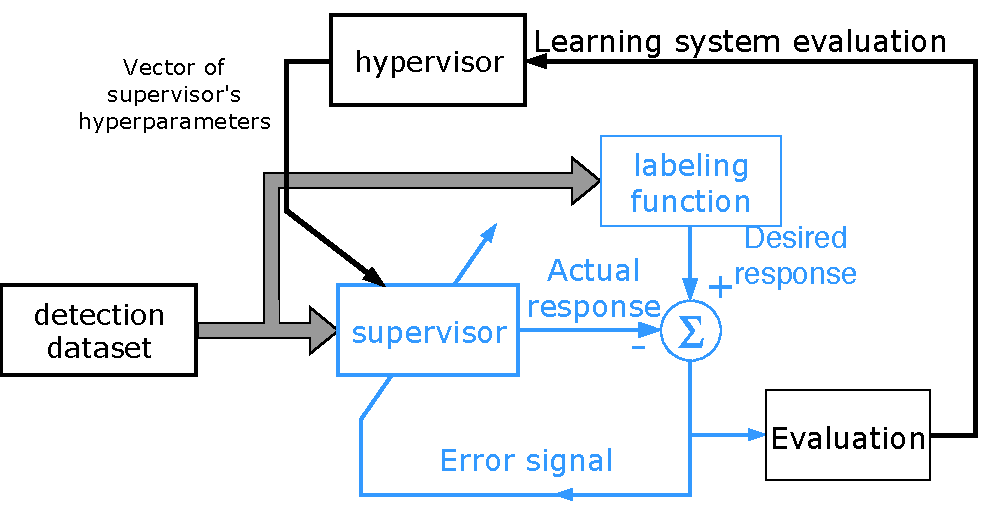
\includegraphics[width = 0.8\textwidth]{figures/architecture/haykin_figure.pdf}
    \caption[Η λειτουργία της υλοποίησης]{Η λειτουργία της υλοποίησης όπως είναι κατά την πορεία της εκπαίδευσης. Ο \textit{supervisor} είναι υπεύθυνος για την εκπαίδευση και βελτιστοποίηση των παραμέτρων του μοντέλου, ενώ ο \textit{hypervisor} είναι υπεύθυνος για τη βελτιστοποίηση των παραμέτρων του \textit{supervisor}.}
    \label{fig:haykin_figure}
\end{figure}

\subsection{supervisor}
Ο \textit{supervisor} είναι υπεύθυνος για την εκπαίδευση του νευρωνικού δικτύου που επιλέγει ο χρήστης. Δηλαδή λαμβάνει ως παραμέτρους το δίκτυο, το σύνολο δεδομένων και όλες τις υπερπαραμέτρους που απαιτούνται κατά την εκπαίδευση από τον \textit{hypervisor} ή τον χρήστη και αναλαμβάνει την συνεχή εκτέλεση του αλγορίθμου back-propagation για το δίκτυο μέχρι αυτό να συγκλίνει στο επιθυμητό οριακό σφάλμα ορισμένο από τον χρήστη ή να αποκλίνει.

Στην πρώτη περίπτωση, επιστρέφονται τα βάρη του δικτύου και ο γράφος της αρχιτεκτονικής του για την ανακατασκευή του. Στη δεύτερη περίπτωση, επιστρέφεται μήνυμα σφάλματος ότι η εκπαίδευση με αυτές τις υπερπαραμέτρους οδηγεί σε αποκλίνουσα συμπεριφορά.

Το σφάλμα το οποίο εξάγεται κατά την διάρκεια της εκπαίδευσης ορίζεται από μία συνάρτηση που αφορά το δίκτυο. Βέβαια, στη παρούσα περίπτωση πρόκειται για την συνάρτηση κόστους του SqueezeDet. Οπότε, δεν αφήνεται περιθώριο για αλλαγές στην εξαγωγή του σφάλματος πέρα από μεταβολή των συντελεστών επιμέρους συντελεστών της συνάρτησης.

Οι υπερπαράμετροι που μπορούν να εισαχθούν για την εκπαίδευση του δικτύου είναι αρκετές. Ωστόσο προκύπτει ότι είναι πιο εύληπτο να εξηγηθούν αυτές, παρά τον πολύπλοκο μηχανισμό που τις υλοποιεί. Παρόλα αυτά, όταν δίνονται οι υπερπαράμετροι σε ένα αρχείο, πιθανόν να περιλαμβάνονται παραπάνω πληροφορίες μέσα στο αρχείο. Οι υπερπαράμετροι που λαμβάνει υπόψιν του το πακέτο \textit{supervisor} είναι οι εξής:

\subsubsection{Λίστα υπερπαραμέτρων}
\begin{itemize}
\setlength{\itemsep}{0pt}
\item \textcolor{LstItemCol}{CLASS\_NAMES} : Τα ονόματα των κλάσεων τα οποία θα κατηγοριοποιηθούν τα εντοπισμένα αντικείμενα.
\item \textcolor{LstItemCol}{CLASSES} : Ο αριθμός των ονομάτων των κλάσεων.
\item \textcolor{LstItemCol}{LEAKY\_COEF} : Παράμετρος διαρροής για τις συναρτήσεις leaky ReLU.
\item \textcolor{LstItemCol}{KEEP\_PROB} : Πιθανότητα να παραμείνει ανεπηρέαστος ένας κόμβος του νευρωνικού δικτύου μετά από εφαρμογή dropout.
\item \textcolor{LstItemCol}{IMAGE\_WIDTH} : Πλάτος εικόνας. Είναι το ίδιο για κάθε εικόνα, αν όχι τότε γίνεται μετατροπή πλάτους της εικόνας εισόδου σε αυτό.
\item \textcolor{LstItemCol}{IMAGE\_HEIGHT} : Ύψος εικόνας. Είναι το ίδιο για κάθε εικόνα, αν όχι τότε γίνεται μετατροπή ύψους της εικόνας εισόδου σε αυτό.
\item \textcolor{LstItemCol}{ANCHOR\_BOX} : Πίνακας ο οποίος εμπεριέχει "anchors" όπως λέγονται στο SqueezeDet \cite{1}, δηλαδή στοιχεία τύπου $(cx,xy,w,h)$, όπου $cx$ η τετμημένη κέντρου του anchor, $cy$ η τεταγμένη κέντρου του anchor, $w$ το πλάτος του anchor και $h$ το ύψος του anchor.
\item \textcolor{LstItemCol}{ANCHORS} : Ο συνολικός αριθμός των anchor
\item \textcolor{LstItemCol}{ANCHOR\_PER\_GRID} : Ο αριθμός των anchor ανά σημείο του τελικού πλέγματος (βλέπε \cite{1}).
\item \textcolor{LstItemCol}{INITIAL\_ANCHOR\_SHAPES} : Πίνακας με προκαθορισμένες τιμές του πλάτους και του ύψους κάθε anchor.
\item \textcolor{LstItemCol}{BATCH\_SIZE} : Μέγεθος της παρτίδας για ευρωστότερη εκπαίδευση, συνίσταται ο αριθμός αυτός να είναι ίσος με 1 για μετεκπαίδευση σε μικρά σετ δεδομένων.
\item \textcolor{LstItemCol}{PROB\_THRESH} : Κατώφλι το οποίο ορίζει αν ένα υποψήφιο εντοπισμένο αντικείμενο θα θεωρηθεί ως ορθό και θα δοθεί ως είσοδο στον αλγόριθμο NMS.
\item \textcolor{LstItemCol}{PLOT\_PROB\_THRESH} : Κατώφλι το οποίο ορίζει αν ένα εντοπισμένο αντικείμενο θα προβληθεί στα αποτελέσματα προς οπτικοποίηση. Χρησιμοποιείται μόνο κατά την οπτικοποίηση των αποτελεσμάτων.
\item \textcolor{LstItemCol}{NMS\_THRESH} : Ανώφλι μετρικής iou μεταξύ των κουτιών που εντοπίστηκαν. Αν δύο κουτιά έχουν μεταξύ τους μεγαλύτερη τιμή iou, τότε κάποιο από αυτά θα αφαιρεθεί όπως προβλέπεται από τον αλγόριθμο NMS.
\item \textcolor{LstItemCol}{TOP\_N\_DETECTION} : Ο μέγιστος αριθμός αντικειμένων τα οποία θα εξαχθούν από μία εικόνα στο πέρα του αλγορίθμου του νευρωνικού δικτύου.
\item \textcolor{LstItemCol}{BGR\_MEANS} : Μέση τιμή του χρώματος των pixel στο σετ δεδομένων σε σειρά BGR ως ένας πίνακας (1, 1, 3).
\item \textcolor{LstItemCol}{LOSS\_COEF\_CONF} : Συντελεστής σφάλματος εμπιστοσύνης παλινδρόμησης.
\item \textcolor{LstItemCol}{LOSS\_COEF\_CLASS} : Συντελεστής σφάλματος παλινδρόμησης της κατηγοριοποίησης.
\item \textcolor{LstItemCol}{LOSS\_COEF\_BBOX} : Συντελεστής σφάλματος παλινδρόμησης του περιβλήματος των υποψήφιων εντοπισμένων αντικειμένων.
\item \textcolor{LstItemCol}{LOSS\_COEF\_CONF\_POS} : Συντελεστής θετικού σφάλματος εμπιστοσύνης για τη παλινδρόμηση του σκορ.
\item \textcolor{LstItemCol}{LOSS\_COEF\_CONF\_NEG} : Συντελεστής αρνητικού σφάλματος εμπιστοσύνης για τη παλινδρόμηση του σκορ. 
\item \textcolor{LstItemCol}{DECAY\_STEPS} : Άριθμος βημάτων κατά τον οποίο γίνεται σμίκρυνση του ρυθμού ανανέωσης βαρών.
\item \textcolor{LstItemCol}{LR\_DECAY\_FACTOR} : Αριθμός με τον οποίο πολλαπλασιάζεται ο ρυθμός μάθησης κάθε \textcolor{LstItemCol}{DECAY\_STEPS} επαναλήψεις.
\item \textcolor{LstItemCol}{LEARNING\_RATE} : Αρχικός ρυθμός μάθησης(ανανέωσης βαρών).
\item \textcolor{LstItemCol}{MOMENTUM} : Ορμή, Χρησιμοποιείται για τον βελτιστοποιητή ορμής \cite{42}.
\item \textcolor{LstItemCol}{BETA1} : Παράμετρος του βελτιστοποιητή Adam beta1.
\item \textcolor{LstItemCol}{BETA2} : Παράμετρος του βελτιστοποιητή Adam beta2.
\item \textcolor{LstItemCol}{WEIGHT\_DECAY} : ποσοστό μείωσης της τιμής του μέτρου των παραμέτρων κατά την ανανέωση τους σε κάθε επανάληψη.
\item \textcolor{LstItemCol}{LOAD\_PRETRAINED\_MODEL} : Αν τα βάρη θα αρχικοποιηθούν όπως στο \cite{1}.
\item \textcolor{LstItemCol}{PRETRAINED\_MODEL\_PATH} : Διαδρομή αρχείου για την αρχικοποίηση του αρχείου. Πρόκειται για αρχείο τύπου \textit{pkl}.
\item \textcolor{LstItemCol}{DEBUG\_MODE} : Ενεργοποίηση ή όχι της λειτουργίας αποσφαλμάτωσης.
\item \textcolor{LstItemCol}{EPSILON} : Πολύ μικρή τιμή για να αποτραπεί η αριθμητική αστάθεια στις πράξεις.
\item \textcolor{LstItemCol}{EXP\_THRESH} : Ανώφλι για τις ασφαλείς εκθετικές συναρτήσεις.
\item \textcolor{LstItemCol}{MAX\_GRAD\_NORM} : Ανώφλι μέτρου παραγώγων. Παράγωγοι με τιμή μεγαλύτερη δε λαμβάνονται υπόψη.
\item \textcolor{LstItemCol}{DATA\_AUGMENTATION} : Αν θα γίνει προσαύξηση των δεδομένων με πρόσθεση θορύβου.
\item \textcolor{LstItemCol}{EXCLUDE\_HARD\_EXAMPLES} : Υπερπαράμετρος που αφορά το σύνολο δεδομένων KITTI.
\item \textcolor{LstItemCol}{BATCH\_NORM\_EPSILON} : Μικρή τιμή που χρησιμοποιείται στους παρονομαστές για τις διαιρέσεις που απαιτεί η εκπαίδευση κατά παρτίδες. Η προκαθορισμένη τιμή είναι αυτή που χρησιμοποιεί και το Caffe framework \cite{101}.
\item \textcolor{LstItemCol}{FREEZE\_LAYERS} : Αντικείμενο που ορίζει για κάθε επίπεδο του νευρωνικού αν θα εκπαιδευτεί ή όχι.
\item \textcolor{LstItemCol}{IS\_TRAINING} : Αν πρόκειται για εκπαίδευση(true) ή απλά για εκτίμηση του μοντέλου(false).
\item \textcolor{LstItemCol}{NUM\_THREAD} : Αριθμός των νημάτων τα οποία εξάγουν δεδομένα από το σετ δεδομένων.
\item \textcolor{LstItemCol}{MAX\_NUM\_PARALLEL\_NETS} : Μέγιστος αριθμός παράλληλων εκπαιδεύσεων.
\item \textcolor{LstItemCol}{PREPROCESS\_DATASET} : Η αληθής τιμή αυτής της υπερπαραμέτρου επιτρέπει την προ-επεξεργασία όλου του σετ δεδομένων και την εξαγωγή των μεταβλητών aidx και deltas για γρηγορότερη εκπαίδευση αργότερα. Ωστόσο, αν η προ-επεξεργασία ενεργοποιηθεί δεν επιτρέπει μοντέλα με διαφορετική αρχιτεκτονική στο επίπεδο που εξάγονται τα anchor.
\end{itemize}

Τέλος, ο υπολογιστικός γράφος του νευρωνικού δικτύου εντοπισμού με βάση αυτή την υλοποίηση φαίνεται στο Σχήμα \ref{fig:computation_graph} στο τέλος του κεφαλαίου. Εκεί γίνονται εμφανείς και περισσότερες λεπτομέρειες της υλοποίησης.

\subsection{hypervisor}
Το πακέτο αυτό είναι υπεύθυνο για το χειρισμό των υπερπαραμέτρων. Στο κύριο μέρος του υλοποιεί έναν αλγόριθμο βελτιστοποίησης μαύρου κουτιού όπως αυτός που περιγράφεται στην ενότητα \ref{section:autohyperparamters}. Αν και στην προαναφερόμενη ενότητα υλοποιείται μόνο ένας από αυτούς, υπάρχει η δυνατότητα επιλογής μεταξύ τεσσάρων αλγορίθμων όπως περιγράφονται στην παρακάτω λίστα.
\begin{enumerate}
    \item random search: Τυχαία αναζήτηση η οποία δοκιμάζει κάθε φορά καινούριες τυχαίες τιμές ως τιμές των παραμέτρων, παραγόμενες από μία γεννήτρια τυχαίων αριθμών.
    \item LIPO: Ο πρώτος αλγόριθμος που παρουσιάζεται στην εργασία του Nicolas και του Cedric \cite{64}. Οι σταθερές $k$ που χρησιμοποιούνται είναι 1, 10, 100. Επίσης ορίζεται μέγιστος αριθμός επαναλήψεων ίσος με 50.
    \item adaLIPO: Ο δεύτερος αλγόριθμος που παρουσιάζεται στην ίδια εργασία. Στη μόνη ρύθμιση που αρκείται είναι στο μέγιστο αριθμό επαναλήψεων (ίσος με 50).
    \item genetic: Ένας τυπικός γενετικός αλγόριθμος σύμφωνα με τις προτάσεις στο \cite{69}. Οι ρυθμίσεις του είναι δίνονται από τον χρήστη.
\end{enumerate}

Την τιμή εκκίνησης και την περιοχή(πλέγμα) στην οποία γίνεται η αναζήτηση της βέλτιστης τιμής των υπερπαραμέτρων την βάζει ο χρήστης για κάθε αλγόριθμο βελτιστοποίησης. Όπως επίσης, εισάγει και τις τιμές ρύθμισης τους αν αυτές απαιτούνται. Εδώ να τονιστεί πως αυτό δεν χρειάζεται για τον αλγόριθμο \textit{adalipo}, αυτό είναι και ένα από τα πλεονεκτήματά του.

Το πακέτο \textit{hypervisor} λαμβάνει ως τιμές τις συνάρτησης βελτιστοποίησης την έξοδο(κύρια μετρική) της διαδικασίας εκτίμησης του μοντέλου. Η μετρική που μελετάται στη συγκεκριμένη περίπτωση είναι η mAP. Η προτίμηση αυτή γίνεται για την καλύτερη σύνδεση με την πρωταρχική εργασία του \textit{SqueezeDet}.

Αν και υπάρχει πληθώρα άλλων πακέτων για αυτή την υλοποίηση, ωστόσο τα υπόλοιπα δεν παρουσιάζονται διότι δεν έχουν μεγάλη σημασία.

\subsection{Περιγραφή πακέτων λογισμικού τρίτων}
Η γλώσσα προγραμματισμού που χρησιμοποιήθηκε ήταν η Python 2.7, διότι είναι πιο πλήρως υποστηριζόμενη από το \textit{Tensorflow}(βλέπε παρακάτω). Το λειτουργικό της συστοιχίας ήταν \textit{Ubuntu 16.04.4 LTS (Xenial Xerus)}. Τα πακέτα που χρησιμοποιήθηκαν στη τελική υλοποίηση δεν ήταν πολλά γιατί όλες οι υπολογιστικές ανάγκες αυτής της εργασίας καλυπτόταν από τις βιβλιοθήκες \textit{Tensorflow} και \textit{NumPy}.

\begin{itemize}
    \item Tensorflow\footnote{\url{https://www.tensorflow.org}} \cite{34}: Ανοικτού κώδικα βιβλιοθήκη για αριθμητικούς υπολογισμούς χρησιμοποιώντας γράφους ροής δεδομένων ανεπτυγμένο από την ερευνητική ομάδα της \textit{Google}. Η ευέλικτη αρχιτεκτονική της επιτρέπει την ανάπτυξη λογισμικού σε μία ή και περισσότερες κεντρικές μονάδες επεξεργασίας CPU ή μονάδες GPU ακόμα και για ενσωματωμένες συσκευές.
    \item NumPy\footnote{\url{http://www.numpy.org}}: Το βασικό πακέτο για επιστημονικούς υπολογισμούς στην Python. Η χρήση του βοήθησε κυρίως στην υλοποίηση του hypervisor, διότι αυτός εκτελείται από τη CPU.
    \item Matplotlib\footnote{\url{https://matplotlib.org/}}: Βιβλιοθήκη της Python για κατασκευή διαγραμμάτων.
    \item Google-Protocol-buffers(protoc)\footnote{\url{https://developers.google.com/protocol-buffers}}: Επεκτάσιμος μηχανισμός της Google για τη σειριοποίηση δομημένων δεδομένων. Ο μηχανισμός αυτός είναι ανεξάρτητος πλατφόρμας, είναι παρόμοιος με αυτόν της XML, ωστόσο μικρότερος και γρηγορότερος. Η κάθε ανάγνωση και συγγραφή γίνεται με συναρτήσεις οι οποίες έχουν παραχθεί από τον μηχανισμό αυτό ειδικά για κάθε περίπτωση. 
    \item vod-converter\footnote{\url{https://github.com/umautobots/vod-converter}}: Εργαλείο για την μετατροπή της μορφής των συνόλων δεδομένων KITTI, PASCAL VOC από το ένα σύνολο δεδομένων στο άλλο. Η παρούσα εργασία συνείσφερε και στην ανάπτυξη αυτού του εργαλείου, πέρα από την χρήση του.
    \item dlib \footnote{\url{http://dlib.net/}} \cite{83}: Βιβλιοθήκη μεθόδων μη γραμμικής βελτιστοποίησης στη C++. Η χρήσης της βοήθησε στην ανάπτυξη και την βελτιστοποίηση της μεθόδου που περιγράφεται στην ενότητα \ref{section:autohyperparamters}.
\end{itemize}

\begin{figure}
    \centering
    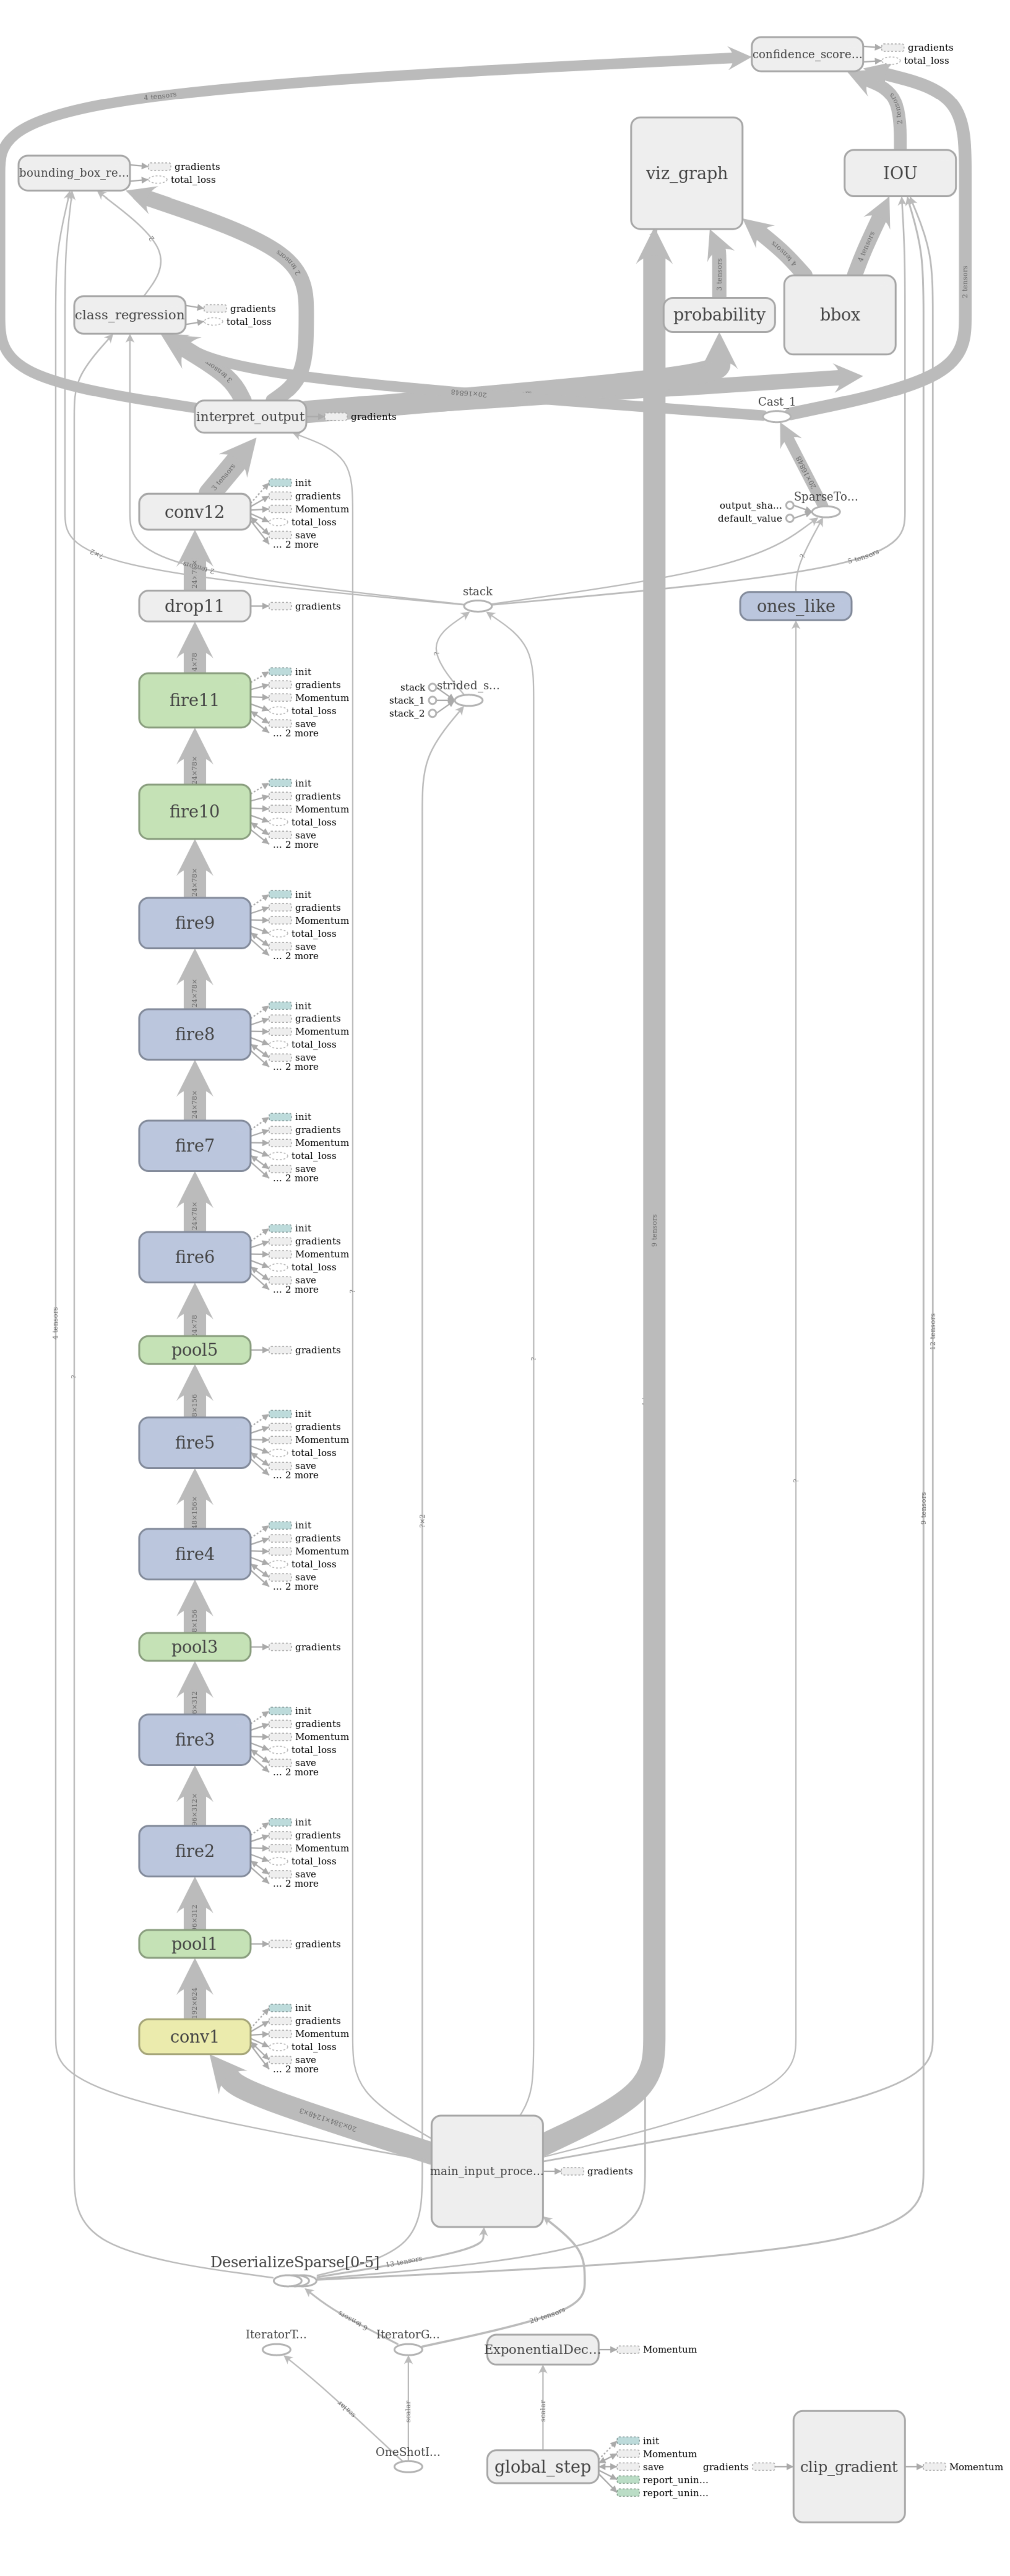
\includegraphics[width=\textwidth,height=\textheight]{figures/architecture/comp_graph.pdf}
    \caption[Ο υπολογιστικός γράφος της υλοποίησης]{Ο υπολογιστικός γράφος της υλοποίησης του SqueezeDet. Το κάθε κομμάτι του γράφου υλοποιεί έναν υπολογισμό. Η πληθώρα αυτών των κομματιών βρίσκεται τοποθετημένη στην GPU. Τα κομμάτια που δεν βρίσκονται στη GPU αφορούν κυρίως την ανάγνωση των δεδομένων από τον δίσκο.}
    \label{fig:computation_graph}
\end{figure}